\newpage
\section{Kunrei System}\jsec{訓令式ローマ字}
% [o] LABEL
\label{sec:Kunrei}
\label{sec:KunreiSystem}
\label{sec:JapanSystemLatinLetters}
% [o] INDEX
\ifor{kunrei system}{訓令式ローマ字}{くんれいろうまじ}{Kunrei System}
\ifor{Japan system Latin letters}{日本式ローマ字}{にほんしきろうまじ}{Lateinische Buchstaben des Japanischen Systems}
\ifor{katakana}{片仮名}{かたかな}{Katakana}
\ifor{hiragana}{平仮名}{ひらがな}{Hiragana}
\ifor{gojūonzu}{五十音図}{ごじゅうおんず}{50@50 Laute Tafel}


% l, r, c, i or o = left, right, center, inner or outer
\begin{wrapfigure}{r}{0.4\textwidth}
        \raisebox{-.5\height}{
        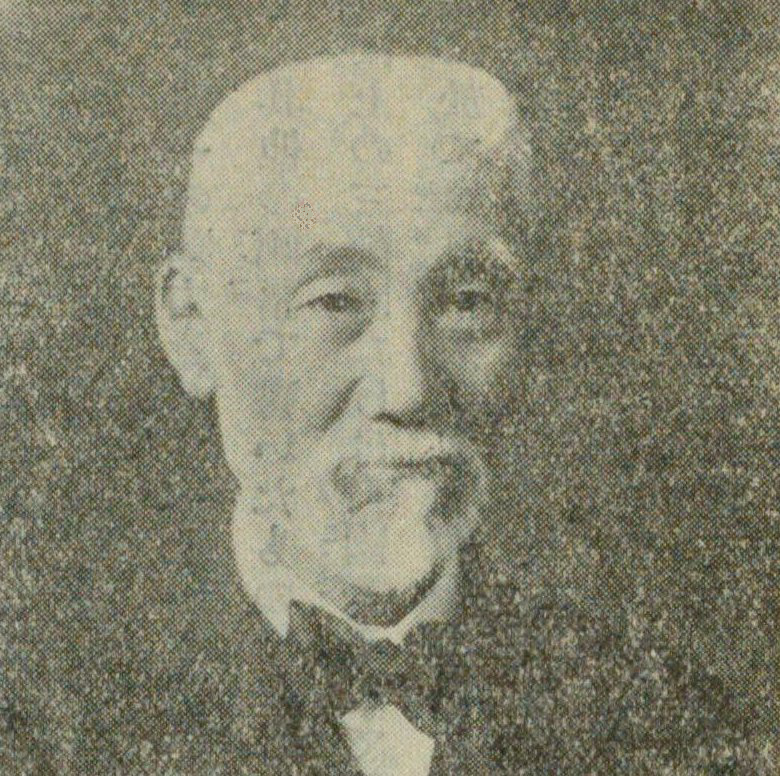
\includegraphics[scale=0.25,trim= 00 00 00 00]{../share/ei/Aikitsu_Tanakadate_r.jpg}}
        \caption{Aikitsu Tanakadate}
        \label{fig:AikitsuTanakadate}
\end{wrapfigure}

The modern \ivoc{kunrei system}{訓令式ローマ字}{くんれいろうまじ}{Kunrei
System} (訓令 = directive; instructions) is the official government-authorized
writing system of Japan, sometimes called \textit{Monbushō system}. It maps
\hyperref[sec:Kana]{kana} (\hyperref[sec:Hiragana]{hiragana} and
\hyperref[sec:Katakana]{katakana}) to \ivoc{rōmaji}{ローマ字}{ろうまじ}{Rōmaji}
(Latin letters). The system was introduced in 1937 and confirmed in 1994 by the
cabinet and is available as ISO 3602:1989.

The \textbf{kunrei system's} predecessor was introduced in 1885 by \Link
\href{https://en.wikipedia.org/wiki/Tanakadate_Aikitsu}{Dr. Aikitsu Tanakadate}
({田中舘愛橘}) as
\ivoc{nihon-/nipponshikiromaji}{日本式ローマ字}{にほんしきろうまじ}{Nihon-/Nipponshikiromaji}
(Japan style Latin letters) known as \textit{Nihonshiki} and tried a more
systematical approach to map \hyperref[sec:Hiragana]{hiragana} and
\hyperref[sec:Katakana]{katakana} to equal Latin letters
(\hyperref[sec:Romaji]{rōmaji}) compared to the \nameref{sec:Hepburn}.

The difference between the \textbf{kunrei system} and the \textit{Nihonshiki}
is that the \textbf{kunrei system} merges the syllable pairs ぢ/じ \jtl{di}/\jtl{zi},
づ/ず \jtl{du}/\jtl{zu}, ぢゃ/じゃ \jtl{dya}/\jtl{zya}, ぢゅ/じゅ \jtl{dyu}/\jtl{zyu}, ぢょ/じょ
\jtl{dyo}/\jtl{zyo}, ゐ/い \jtl{wi}/\jtl{i}, ゑ/え \jtl{we}/\jtl{e}, くゎ/か \jtl{kwa}/\jtl{ka}, and ぐゎ/が
\jtl{gwa}/\jtl{ga} as the pronunciation is now identical in modern Japanese.

However, the modern \hyperref[sec:Gojuonzu]{gojūonzu} in the \textbf{kunrei
system} is as follows:

\Info{訓令式ローマ字 - Kunrei System}{
\begin{center}
\begin{tabular}{|c|c|c|c|c|}\hline
   a & i& u& e& o\\\hline
   ka&ki&ku&ke&ko\\\hline
   sa&si&su&se&so\\\hline
   ta&ti&tu&te&to\\\hline
   na&ni&nu&ne&no\\\hline
   ha&hi&hu&he&ho\\\hline
   ma&mi&mu&me&mo\\\hline
   ya&  &yu&  &yo\\\hline
   ra&ri&ru&re&ro\\\hline
   wa&  &  &  & o\\\hline
     &  &  &  & n\\\hline
\end{tabular}
\end{center}
}{true}

Even tough the system is official, many entities (like the train system) or
even the Japanese state is not using it always. Sometimes they use the Hepburn
system. The Japanese state uses the Hepburn system for passports and road
signs, the train system use the Hapburn system for station names for example.

The \textbf{kunrei system} is not used in this book and therefore not part of
this book. Please see \nameref{sec:Hepburn} (on page \pageref{sec:Hepburn}) for
the system used in this book.
